\section{The Source Metamodel}
\label{sec:sourcemetamodel}

The source language is authored in two documents that together form one
metamodel. A \emph{project} document is written by the owner of a group of
applications and states what those applications need. A single \emph{platform}
document is written once for the estate and states what the estate offers. The
split follows directly from the contention rule of Section~\ref{sec:decisions}:
a value that must be unique across the estate, or that draws on a shared finite
resource, is stated in the platform document, and everything else is stated by
the application that needs it.

\subsection{The Project Document}

Figure~\ref{fig:sourcemetamodel} shows the project half of the source
metamodel. Its root is a \texttt{Project}, which carries an owner and the
applications it groups. An \texttt{Application} is the unit that is released as
a whole: it carries an identifier that is unique across the estate, the
processes released together, the hostnames it is reachable at, the secrets it
holds, how its database schema moves when a new version replaces the old one,
and, optionally, how its failures should be alerted.

A \texttt{Migration} is a union of three answers. A \texttt{ManagedMigration}
names a Liquibase changelog, by its path in the application's repository, that
the platform's runner applies before any new version starts. A
\texttt{SelfMigration} says the image migrates its own schema, which is the only
honest answer for a third-party image. A \texttt{NoMigration} says the
application moves no schema, because another application of the same project
does. The answer is required exactly where an application reaches a database,
and one application of a project moves that project's one database.

% Every figure is cut from the one mermaid block that mirrors the metamodel,
% by scripts/diagrams/class-diagram.py, so no part can drift from the whole.
\begin{figure}[!htbp]
\centering
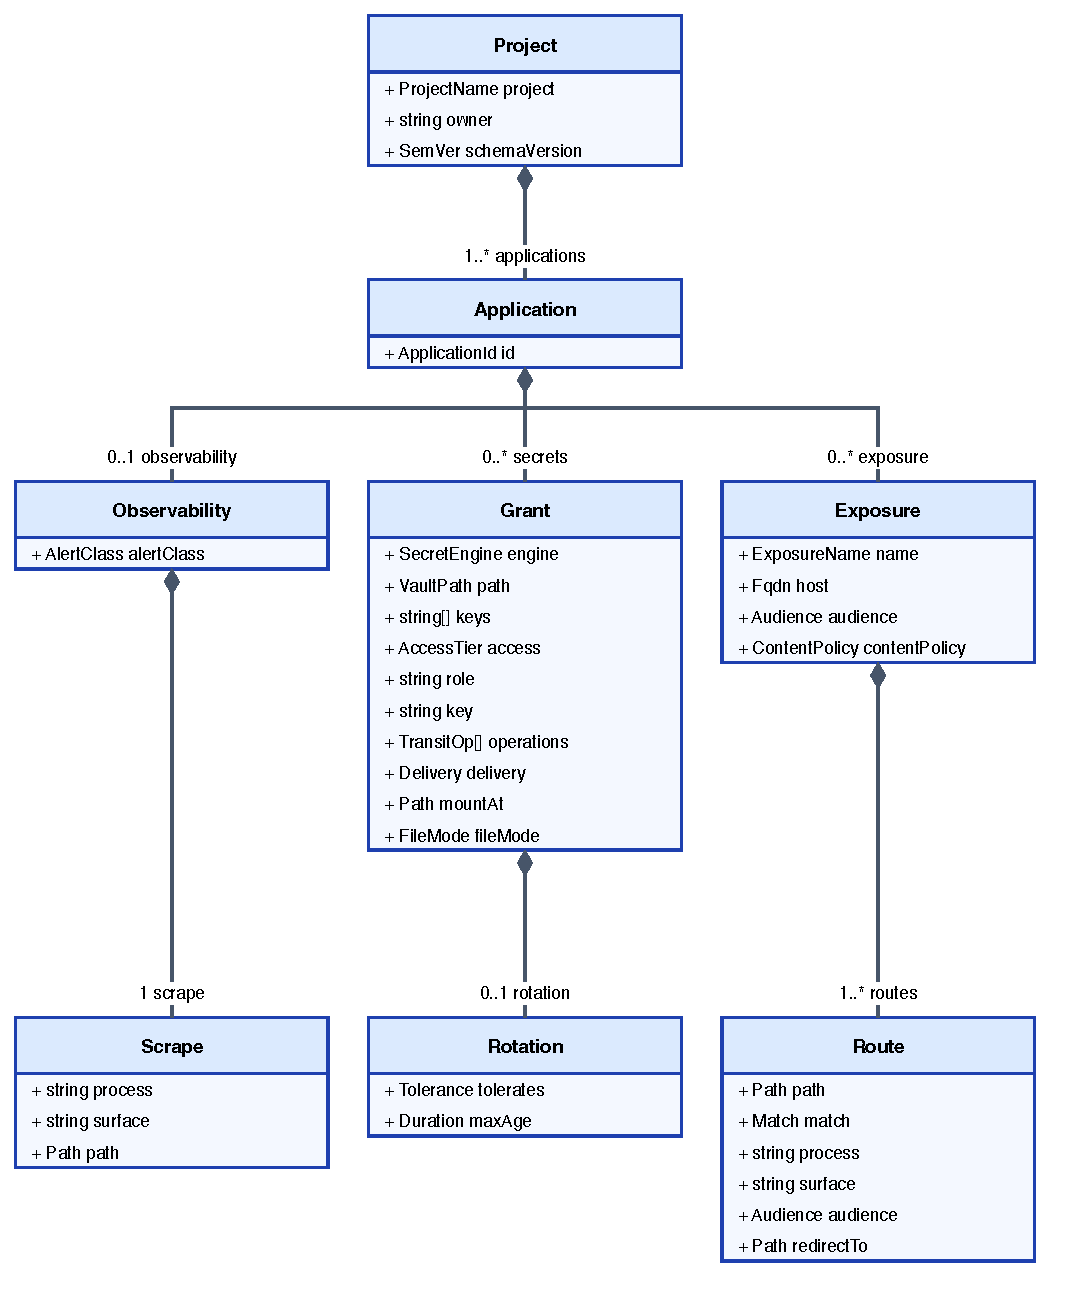
\includegraphics[width=0.92\linewidth, keepaspectratio]{Figures/s-app}
\caption{The Project Document: the Application and What Belongs to It}
\label{fig:sourcemetamodel}
\end{figure}

A \texttt{Process} is the level at which almost every operational concern sits.
It names the image it runs, what kind of thing it is, which named ports it
offers, what it needs from a machine, which paths it must write, what answers a
health check, what its volumes are worth, and whether it must keep serving while
a new version replaces it. That last answer is its \emph{cutover}:
\texttt{continuous} asks for the new version to start beside the old one and take
traffic only once every process of the application has passed analysis, and
\texttt{interrupted} accepts a stop-then-start. A process's kind is one of
\texttt{application}, \texttt{job}, or \texttt{prepare}: a prepare process is
forward-only setup, such as a seed, that runs to completion after the migration
and before the new version starts, and serves nothing. The concerns that belong to the application
rather than to one of its processes are kept on the application: a hostname
fronts several processes and picks between them by path, so exposure cannot sit
on a process without being written twice.


A \texttt{Process} carries almost every operational concern, so it is shown in
four figures rather than one: Figure~\ref{fig:sourceprocess1} its capacity,
helpers and health, Figure~\ref{fig:sourceplacement} what it needs from a
machine, Figure~\ref{fig:sourceprocess2} its storage and files, and
Figure~\ref{fig:sourceprocess3} its configuration, dependencies and the ports
it offers. All four are cut from the same source as
Figure~\ref{fig:sourcemetamodel}.

\begin{figure}[!htbp]
\centering
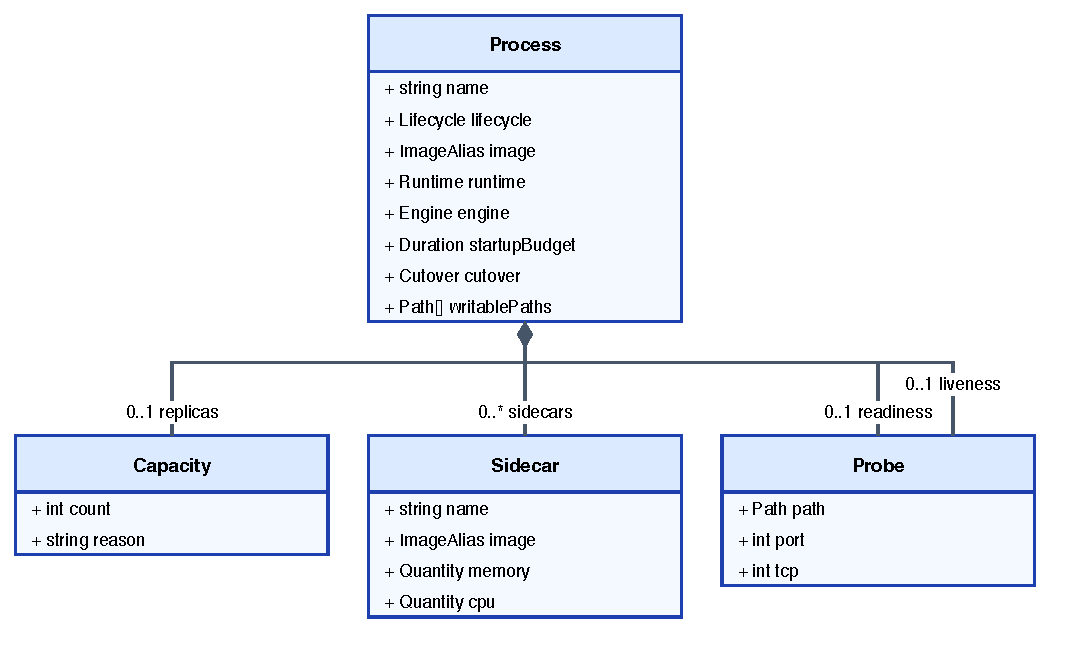
\includegraphics[width=0.92\linewidth, keepaspectratio]{Figures/s-proc-a}
\caption{A Process: Capacity, Helpers and Health}
\label{fig:sourceprocess1}
\end{figure}
\begin{figure}[!htbp]
\centering
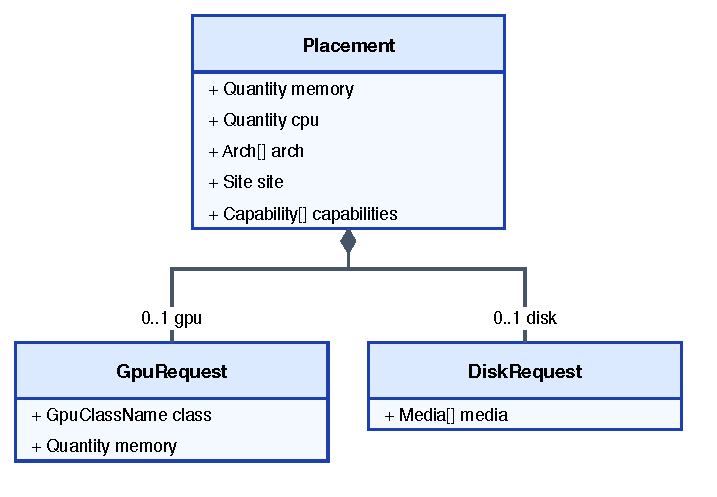
\includegraphics[width=0.92\linewidth, keepaspectratio]{Figures/s-place}
\caption{A Process: What It Needs From a Machine}
\label{fig:sourceplacement}
\end{figure}
\begin{figure}[!htbp]
\centering
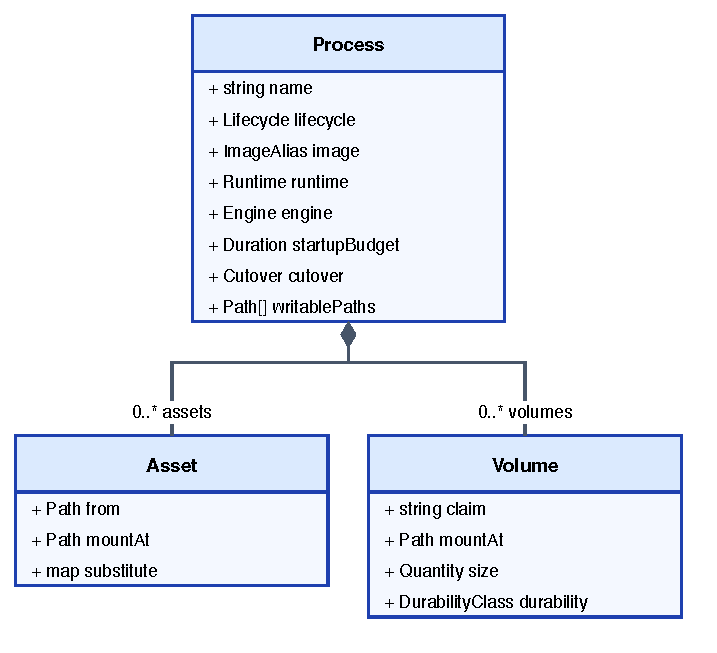
\includegraphics[width=0.92\linewidth, keepaspectratio]{Figures/s-proc-b}
\caption{A Process: Storage and Files}
\label{fig:sourceprocess2}
\end{figure}
\begin{figure}[!htbp]
\centering
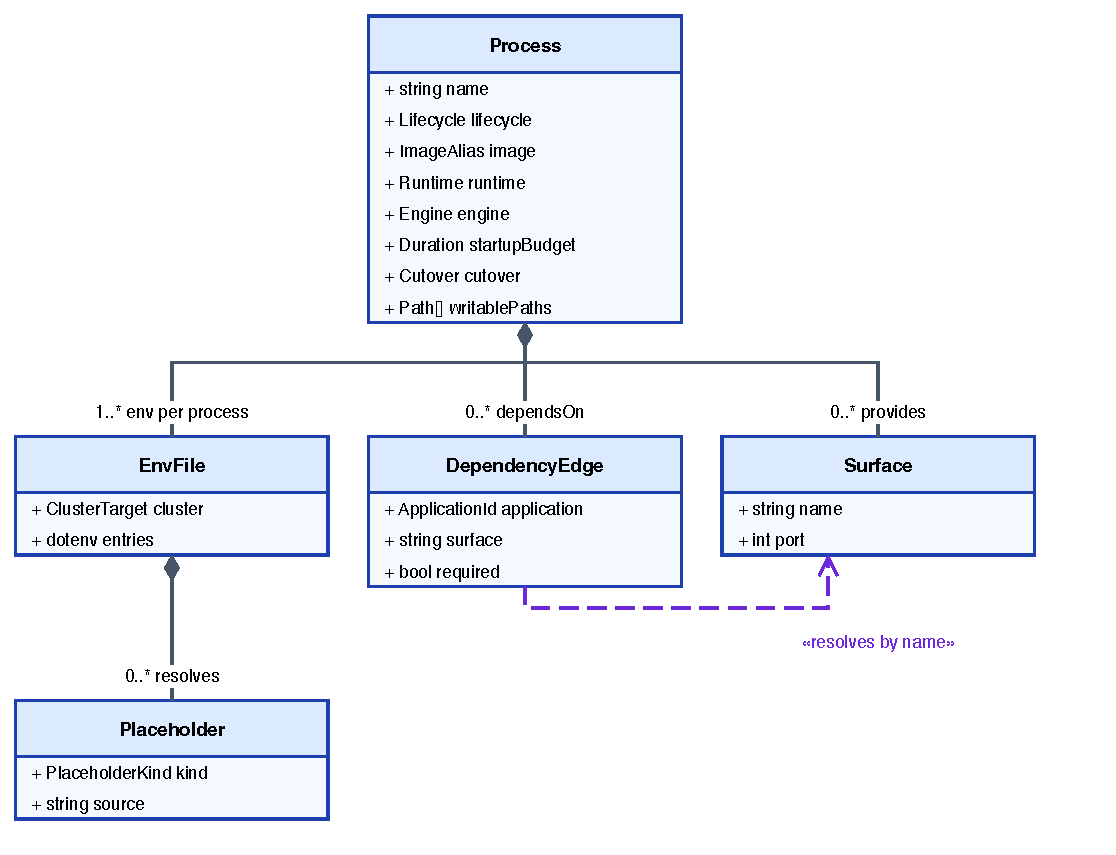
\includegraphics[width=0.92\linewidth, keepaspectratio]{Figures/s-proc-c}
\caption{A Process: Configuration, Dependencies and the Ports It Offers}
\label{fig:sourceprocess3}
\end{figure}

Table~\ref{tab:sourceclasses} lists the classes and what each one is for.

\begin{table}[!htbp]
\centering
\small
\begin{tabular}{>{\raggedright\arraybackslash}p{0.22\linewidth}>{\raggedright\arraybackslash}p{0.70\linewidth}}
\hline
\textbf{Class} & \textbf{What it represents} \\
\hline
Project & The authored unit: an owner and the applications the document groups. \\
Application & What is released as a whole, identified uniquely across the estate. \\
Process & One containerised process: image, kind, ports, needs and health. \\
Surface & A named port a process offers, declared once. \\
Exposure & A hostname the application is reachable at, and who may reach it. \\
Route & A path on that hostname, and the process and surface that serve it. \\
Placement & What a process needs from a machine, as hard requirements. \\
Volume & Storage a process holds, with what its data is worth if lost. \\
Probe & What answers readiness or liveness for a process. \\
Dependency & An edge to another application's named surface, carrying, where the provider owns databases, how the credential it derives may rotate. \\
Credentials & The rotation an application can honour for the database credential its edge derives. \\
Migration & How the application's schema moves: a Liquibase changelog the platform applies, the image itself, or nothing. \\
Grant & A secret a process may read, how it is delivered, and its rotation. \\
Asset & A file a process needs that is configuration rather than code. \\
Observability & Where metrics are collected and how urgently failures alert. \\
Sidecar & A helper process sharing the main process's lifetime. \\
Capacity & A count above one, with the reason it is not derived. \\
\hline
\end{tabular}
\caption{Classes of the Project Document}
\label{tab:sourceclasses}
\end{table}

\subsection{The Platform Document}

The platform document carries the facts and policies that no single application
may decide: what the cluster is, where the edge terminates and which audiences
each edge tier serves, one backup policy per durability class, one backup method
per engine, one hardening posture, one probe cadence, one monitoring cadence,
the services the estate runs without deploying them, the runner every managed
migration builds on, how a release is switched: which applications perform
the switch and are never switched by it, and the cadence at which a new version
is analysed, where each project's rendered output is published and whose
signature the cluster accepts on it, and, while the estate moves off its old
delivery path, which path each project is on.

It is shown in four figures, cut from its own source by the same script that
cuts the project half. Figure~\ref{fig:platformfacts} holds the facts about the
cluster and what must exist before a rendered object can land, including where
the reconciler fetches each project's rendered output and whose keyless
signature it verifies,
Figure~\ref{fig:platformedge} the edge and what the estate already runs, and
Figure~\ref{fig:platformpolicies} the policies: one per durability class, one
per engine, and the cadences the derivations read. Figure~\ref{fig:platformdelivery}
holds what delivery reads: the migration runner and its terms, the delivery
machinery with its analysis cadence, and the handover ledger.

\begin{figure}[!htbp]
\centering
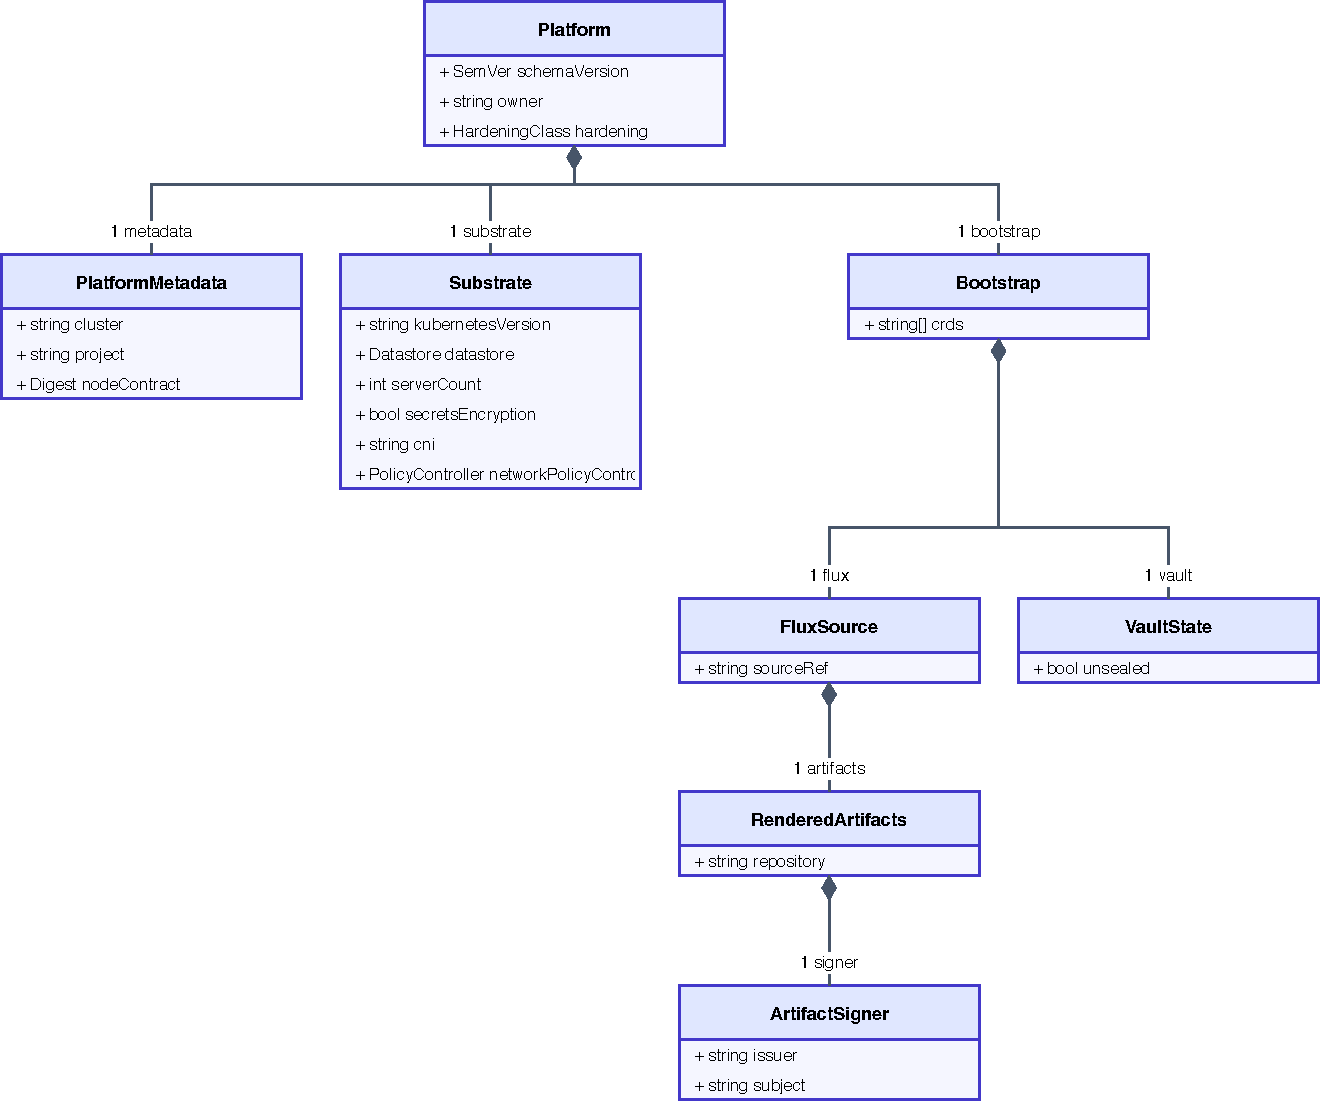
\includegraphics[width=0.78\linewidth, keepaspectratio]{Figures/s-plat-a}
\caption{The Platform Document: the Cluster and What Must Already Exist}
\label{fig:platformfacts}
\end{figure}
\begin{figure}[!htbp]
\centering
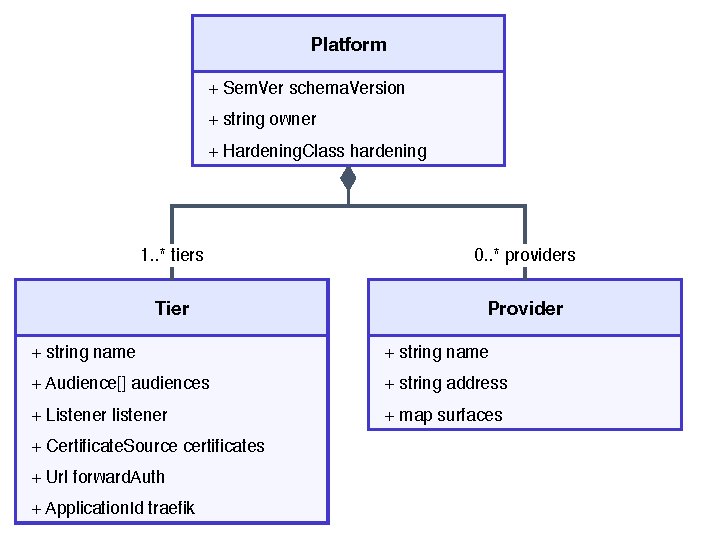
\includegraphics[width=0.50\linewidth, keepaspectratio]{Figures/s-plat-b}
\caption{The Platform Document: the Edge, and What the Estate Already Runs}
\label{fig:platformedge}
\end{figure}
\begin{figure}[!htbp]
\centering
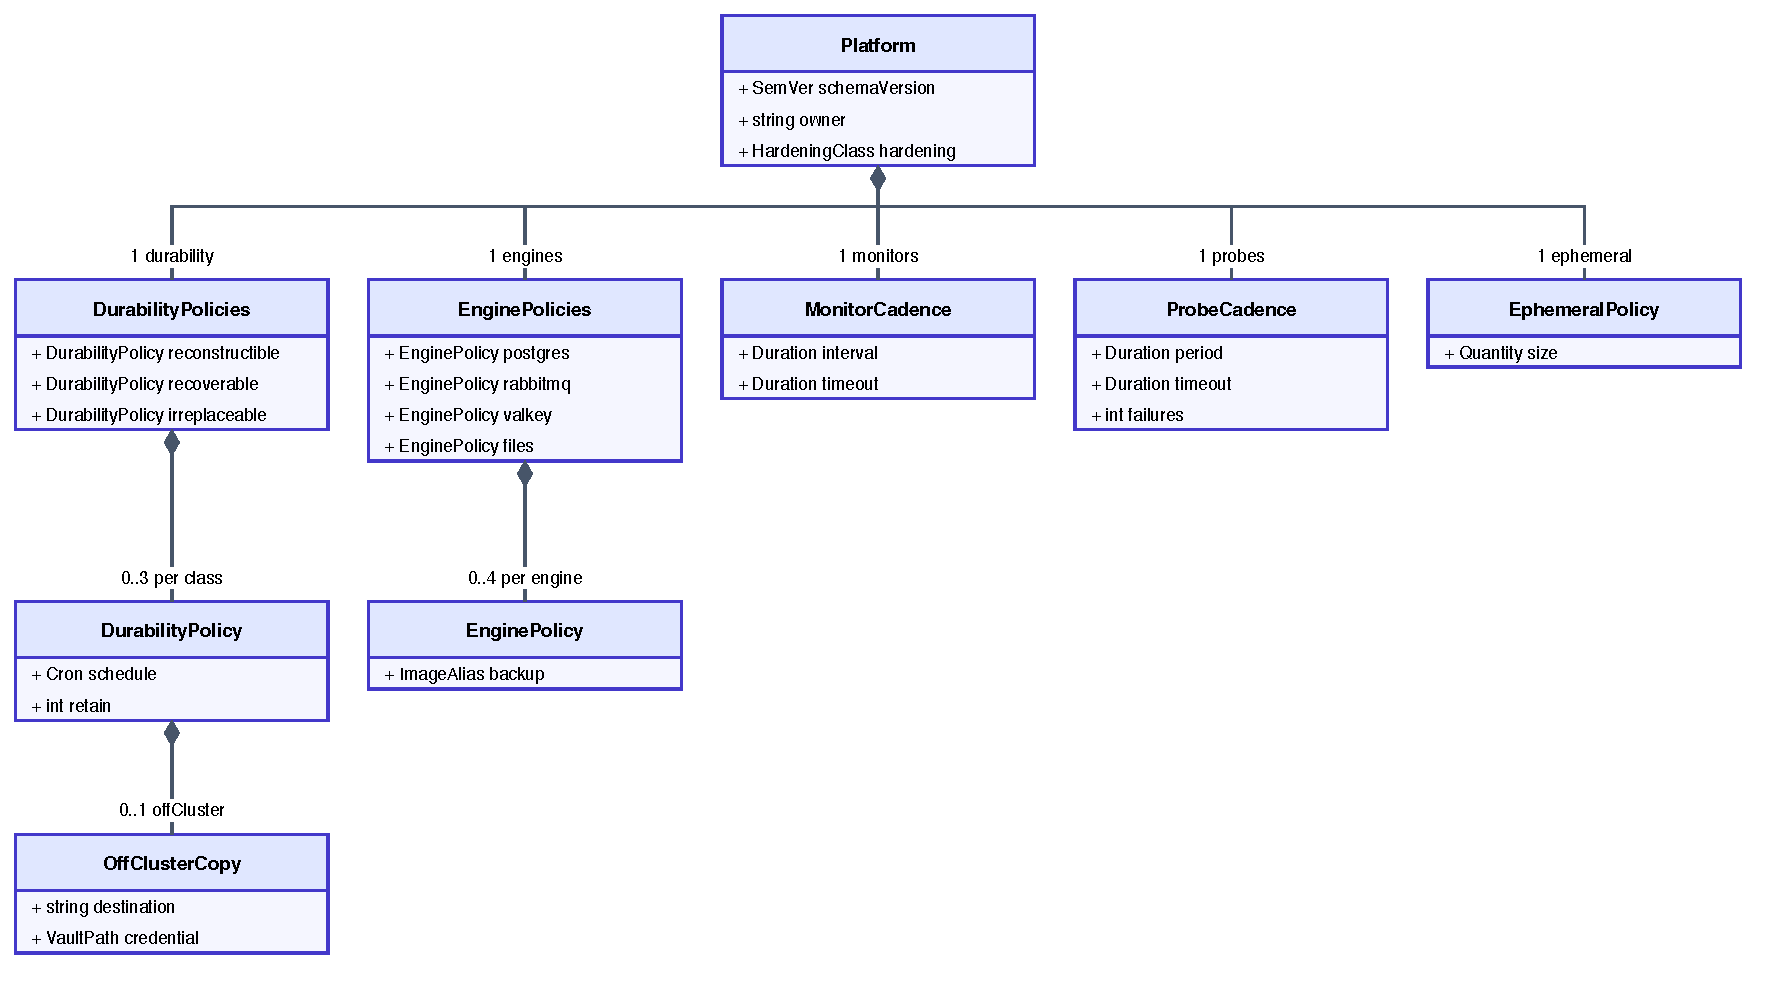
\includegraphics[width=0.92\linewidth, keepaspectratio]{Figures/s-plat-c}
\caption{The Platform Document: the Policies a Derivation Reads}
\label{fig:platformpolicies}
\end{figure}
\begin{figure}[!htbp]
\centering
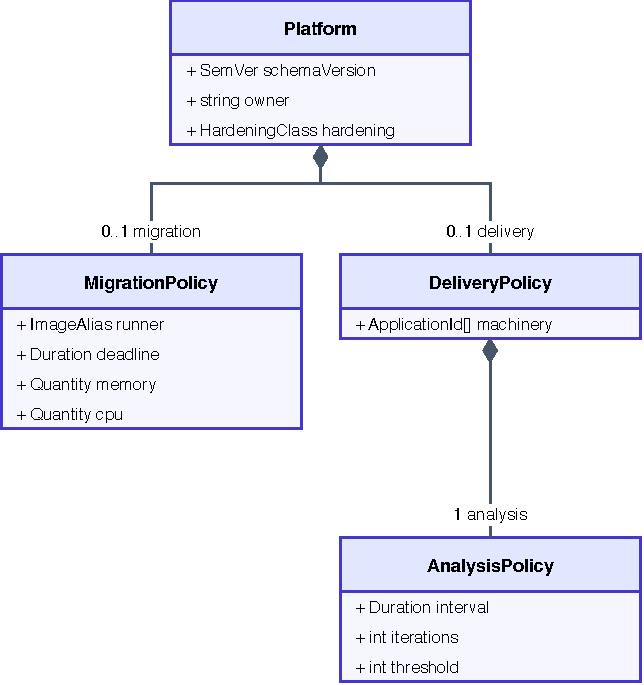
\includegraphics[width=0.72\linewidth, keepaspectratio]{Figures/s-plat-d}
\caption{The Platform Document: What Delivery Reads}
\label{fig:platformdelivery}
\end{figure}

A fact here is named for what it is and never for how the cluster is told about
it, which is the rule of Section~\ref{sec:decisions} applied to the document
that is most tempted to break it. Two of these facts gate a constraint rather
than feed a derivation: a cluster that does not encrypt secrets at rest refuses
every delivery that would write one into it, and a durability class or an engine
with no policy refuses the volume or the process that asked for it
(Section~\ref{sec:constraints}).

Table~\ref{tab:platformclasses} lists the classes.

\begin{table}[!htbp]
\centering
\small
\begin{tabular}{>{\raggedright\arraybackslash}p{0.22\linewidth}>{\raggedright\arraybackslash}p{0.70\linewidth}}
\hline
\textbf{Class} & \textbf{What it represents} \\
\hline
Platform & The estate-wide authored document: one per cluster, with its owner and hardening posture. \\
PlatformMetadata & Which cluster and project the document describes, and the digest of the machine contract it was written against. \\
Substrate & Facts about the cluster that decide other decisions: its version, datastore, server count, whether secrets are encrypted at rest, and its network plugin and policy controller. \\
Bootstrap & What must already exist before the first rendered object can land, recorded rather than declared. \\
FluxSource & The reconciler's source reference, part of that bootstrap set. \\
RenderedArtifacts & The registry repository each project's rendered output is published to, one signed artifact per project. \\
ArtifactSigner & The keyless identity, an issuer and a subject, whose signature the reconciler accepts on a rendered artifact. \\
VaultState & Whether the secret store is unsealed, the second bootstrap fact. \\
Tier & Where the edge terminates: the audiences it serves, its listener, its certificate source, the endpoint that decides an authenticated request, and the declared Application that is its proxy. \\
DurabilityPolicies & The three durability classes' policies, held together so a missing one is visible. \\
DurabilityPolicy & One class's backup window and retention. \\
OffClusterCopy & Where an irreplaceable volume's copy goes, and the credential that writes it. \\
EnginePolicies & The backup method per engine, held together for the same reason. \\
EnginePolicy & One engine's backup image alias, named and never executable. \\
MonitorCadence & How often the estate collects metrics, and how long it waits. \\
ProbeCadence & The estate's one probe cadence: period, timeout and the failures tolerated. \\
EphemeralPolicy & The size a declared writable path receives. \\
Provider & Something the estate runs and this model does not deploy, with its address and named surfaces, which a dependency may resolve against. \\
MigrationPolicy & The runner image alias every managed migration builds on, with the deadline and resources its run takes. \\
DeliveryPolicy & The applications that perform a switch and are never switched by one, linked across documents like a tier's proxy. \\
AnalysisPolicy & How often a new version is checked, how many passing checks promote it, and how many failing ones roll it back. \\
HandoverLedger & While the estate moves off its old delivery path: the projects still delivered by it, the projects delivered by their pin, and the date the old path is removed. \\
\hline
\end{tabular}
\caption{Classes of the Platform Document}
\label{tab:platformclasses}
\end{table}

\subsection{Closed Vocabularies}

Wherever an attribute admits a fixed set of values, the metamodel declares an
enumeration. The project document contributes vocabularies for the kind of a
process (\texttt{application}, \texttt{job}, \texttt{prepare}), its runtime, its
engine, its cutover (\texttt{continuous} or \texttt{interrupted}), a volume's durability
class, machine architecture and storage medium, alert urgency, the audience of
an exposure, a content policy, a path match, a secret's access tier and
delivery, and a rotation tolerance. The platform document contributes
vocabularies for the cluster's datastore and policy controller, an edge tier's
listener and certificate source, and the hardening class.

The enumerations are the surface most of the constraints are written against,
which is the argument of Section~\ref{sec:alternatives} against free-form
properties: a constraint can enumerate an enumeration exhaustively, and cannot
enumerate a string.
